

\section{Physics in the Hadron Collision}
\label{sec:relatedWorks:ppCollision} 

When protons collide in the hadron colliders, it is actually the quarks and gluons inside the protons, called partons, that collide at the high center-of-mass energy. This high energy collision of partons is called the hard process and can be calculated perturbatively with QFT. However, the outcoming result of the proton-proton collision not only involves the physics in the hard process, but also includes many low-energy QCD processes happening before and after the hard process that cannot be treated with perturbative QCD. Therefore to properly make predictions on the hadron collider experiments, efforts are made to understand how partons distribute in the collided protons before the hard process and how outcoming particles evolve in the long-distance range after the hard process. These studies yield the topics of PDF and jet physics. In this section, a brief description of the PDF, hard process, and jet physics are presented. Such a description provides a basic theoretical foundation to understand the Monte Carlo simulations with modern event generators. Also, it helps understand the source of the theoretical systematical uncertainties in the $Br(W)$ analysis.

\subsection{Parton Distribution Function}
\label{sec:relatedWorks:ppCollision:pdf} 


A proton is formed of partons, which include valence quarks, sea quarks, and gluons. It can be pictured as three valence quarks surrounded by a cloud of soft gluon and sea quarks. For a proton with a given momentum, the probability distribution of a certain type of parton is described by the Parton Distribution Function (PDF) $f_i(x)$, where $x$ denotes the fraction of the total proton momentum $p$ carried by the parton. When colliding protons, partons are actually participating in the high energy hard process. As a result, the collision cross-section is a convolution of the cross-section of the hard process with the two PDFs of the interacting partons:
\begin{equation}
    \sigma_{pp\to X } = \sum_{ij}\int dx_1 dx_2 f_i(x_1, \mu^2) f_j(x_2, \mu^2) \hat{\sigma}_{ij\to X } (x_1 p_1, x_2 p_2,\mu^2) .
    \label{eqn:relatedWorks:qft:ppCollision:factorization}
\end{equation}

\noindent This \textbf{factorizes} the total cross-section into the hard collision and PDFs, where $\mu$ is the factorization scale. To make theoretical predictions to experimental data, the theoretical model needs external input about the PDF, which is primarily measured in the lepton-hadron deep inelastic scattering (DIS) experiments. The DIS cross-section yields the structure functions of the hadrons $F_2(x)$, which theoretically equals to the sum of PDF weighted by the quark momentum and charge squared: $F_2(x) = \sum_i x Q^2_i f_i(x)$. The PDFs of different quarks $f_i(x)$ are extracted from DIS with protons and neutron targets, using the quark symmetries of the proton and neutron. The PDFs of anti-quarks are extracted from DIS with neutrino and anti-neutrino beams because the intermediating $W^\pm$ boson is capable of probing specific charge conjugated states, either quarks or anti-quarks. However, the gluon distribution is not directly measured in the DIS experiment because both the intermediating photon and W boson in the DIS do not carry colors and do not probe the gluons inside the proton. Instead, gluon information is indirectly extracted from the PDF evolution in different energy scales based on the DGLAP equation:
\begin{equation}
    \mu \frac{d}{d\mu} \begin{bmatrix} f_i(x,\mu) \\ f_g(x,\mu) \end{bmatrix} = 
    \sum_j \frac{\alpha_s}{\pi} \int_x^1 
    \frac{dy}{y}
    \begin{bmatrix} P_{q_i q_j}(\frac{x}{y}) & P_{q_i g}(\frac{x}{y}) \\ P_{g q_j}(\frac{x}{y}) & P_{gg}(\frac{x}{y})) \end{bmatrix} \begin{bmatrix} f_j(y,\mu) \\ f_g(y,\mu) \end{bmatrix} ,
    \label{eqn:relatedWorks:qft:ppCollision:dglap}
\end{equation}

\noindent where $P_{ab}$ is the DGLAP splitting function, representing the probability of parton $a$ radiating another parton $b$ with the fraction momentum $z=\frac{p_b}{p_a}$. The splitting  functions $P_{ab}$ are calculated by considering the tree-level Feynman diagram and reads as
\begin{equation}
\begin{split}
	P_{qq}(z) &= \frac{4}{3}\bigg[\frac{1+z^2}{1-z} \bigg]_+, P_{qg}(z)=\frac{1}{2} \bigg[z^2+(1-z)^2 \bigg], P_{gq}(z)=\frac{4}{3}\bigg[\frac{1+(1-z)^2}{z} \bigg]\\
    P_{gg}(z) &= 6 \bigg[ \frac{z}{1-z}_+ + \frac{1-z}{z} + z(1-z) \bigg] +(11-\frac{n_f}{3})\delta(1-z) .
\end{split}
\label{eqn:relatedWorks:qft:ppCollision:splitting}
\end{equation}

\noindent The DGLAP equation is a renormalization group equation for the scale-dependent PDF evolution, similar to the RGE for the running of coupling in Equation~\ref{eqn:relatedWorks:qft:qcd:rge}. The driven source for the PDF evolution is the splitting functions in Equation~\ref{eqn:relatedWorks:qft:ppCollision:splitting}, analogical to the role of beta function in the running of coupling.  An intuitive understanding of the PDF evolution is that as the probing energy increases, more and more ``soft cloud" of sea quarks and gluons are revealed. As a result, the PDFs of sea quarks and gluons increase in the low $x$ region. Since gluons dominate the soft cloud, the PDF evolution tells information about the gluon PDF, given that the quark PDFs are known from DIS. The DGLAP equation in Equation~\ref{eqn:relatedWorks:qft:ppCollision:dglap} is a set of two first-order linear differential equations, and the solution is
\begin{equation}
    \begin{bmatrix} f_i(x,\mu^2) \\ f_g(x,\mu^2) \end{bmatrix} = \begin{bmatrix} f_i(x) \\ f_g(x) \end{bmatrix} + 
    \frac{\alpha_s}{2\pi} \log\bigg(\frac{\mu^2}{\mu_0^2}\bigg) 
    \sum_j \int_x^1 
    \frac{dy}{y}
    \begin{bmatrix} P_{q_i q_j}(\frac{x}{y}) & P_{q_i g}(\frac{x}{y}) \\ P_{g q_j}(\frac{x}{y}) & P_{gg}(\frac{x}{y})) \end{bmatrix} \begin{bmatrix} f_j(y) \\ f_g(y) \end{bmatrix}  , 
\end{equation}

\noindent where the $\mu^2$ is the variable factorization scale in Equation~\ref{eqn:relatedWorks:qft:ppCollision:factorization}, and $\mu^2_0$ is the reference scale of the renormalization group. The measured PDFs at two different energy scales  $\mu^2=10 \text{ GeV}^2$ and $\mu^2=10^4 \text{ GeV}^2$ are shown in Figure~\ref{fig:relatedWorks:ppCollision:pdf}

% The parton splitting in the initial state radiation is IR divergent. We introduce a factorization scale and DGLAP integrates the non-perturbation physics in PDF, leaving had scattering fully perterbative. 

\begin{figure}[ht]
    \centering
    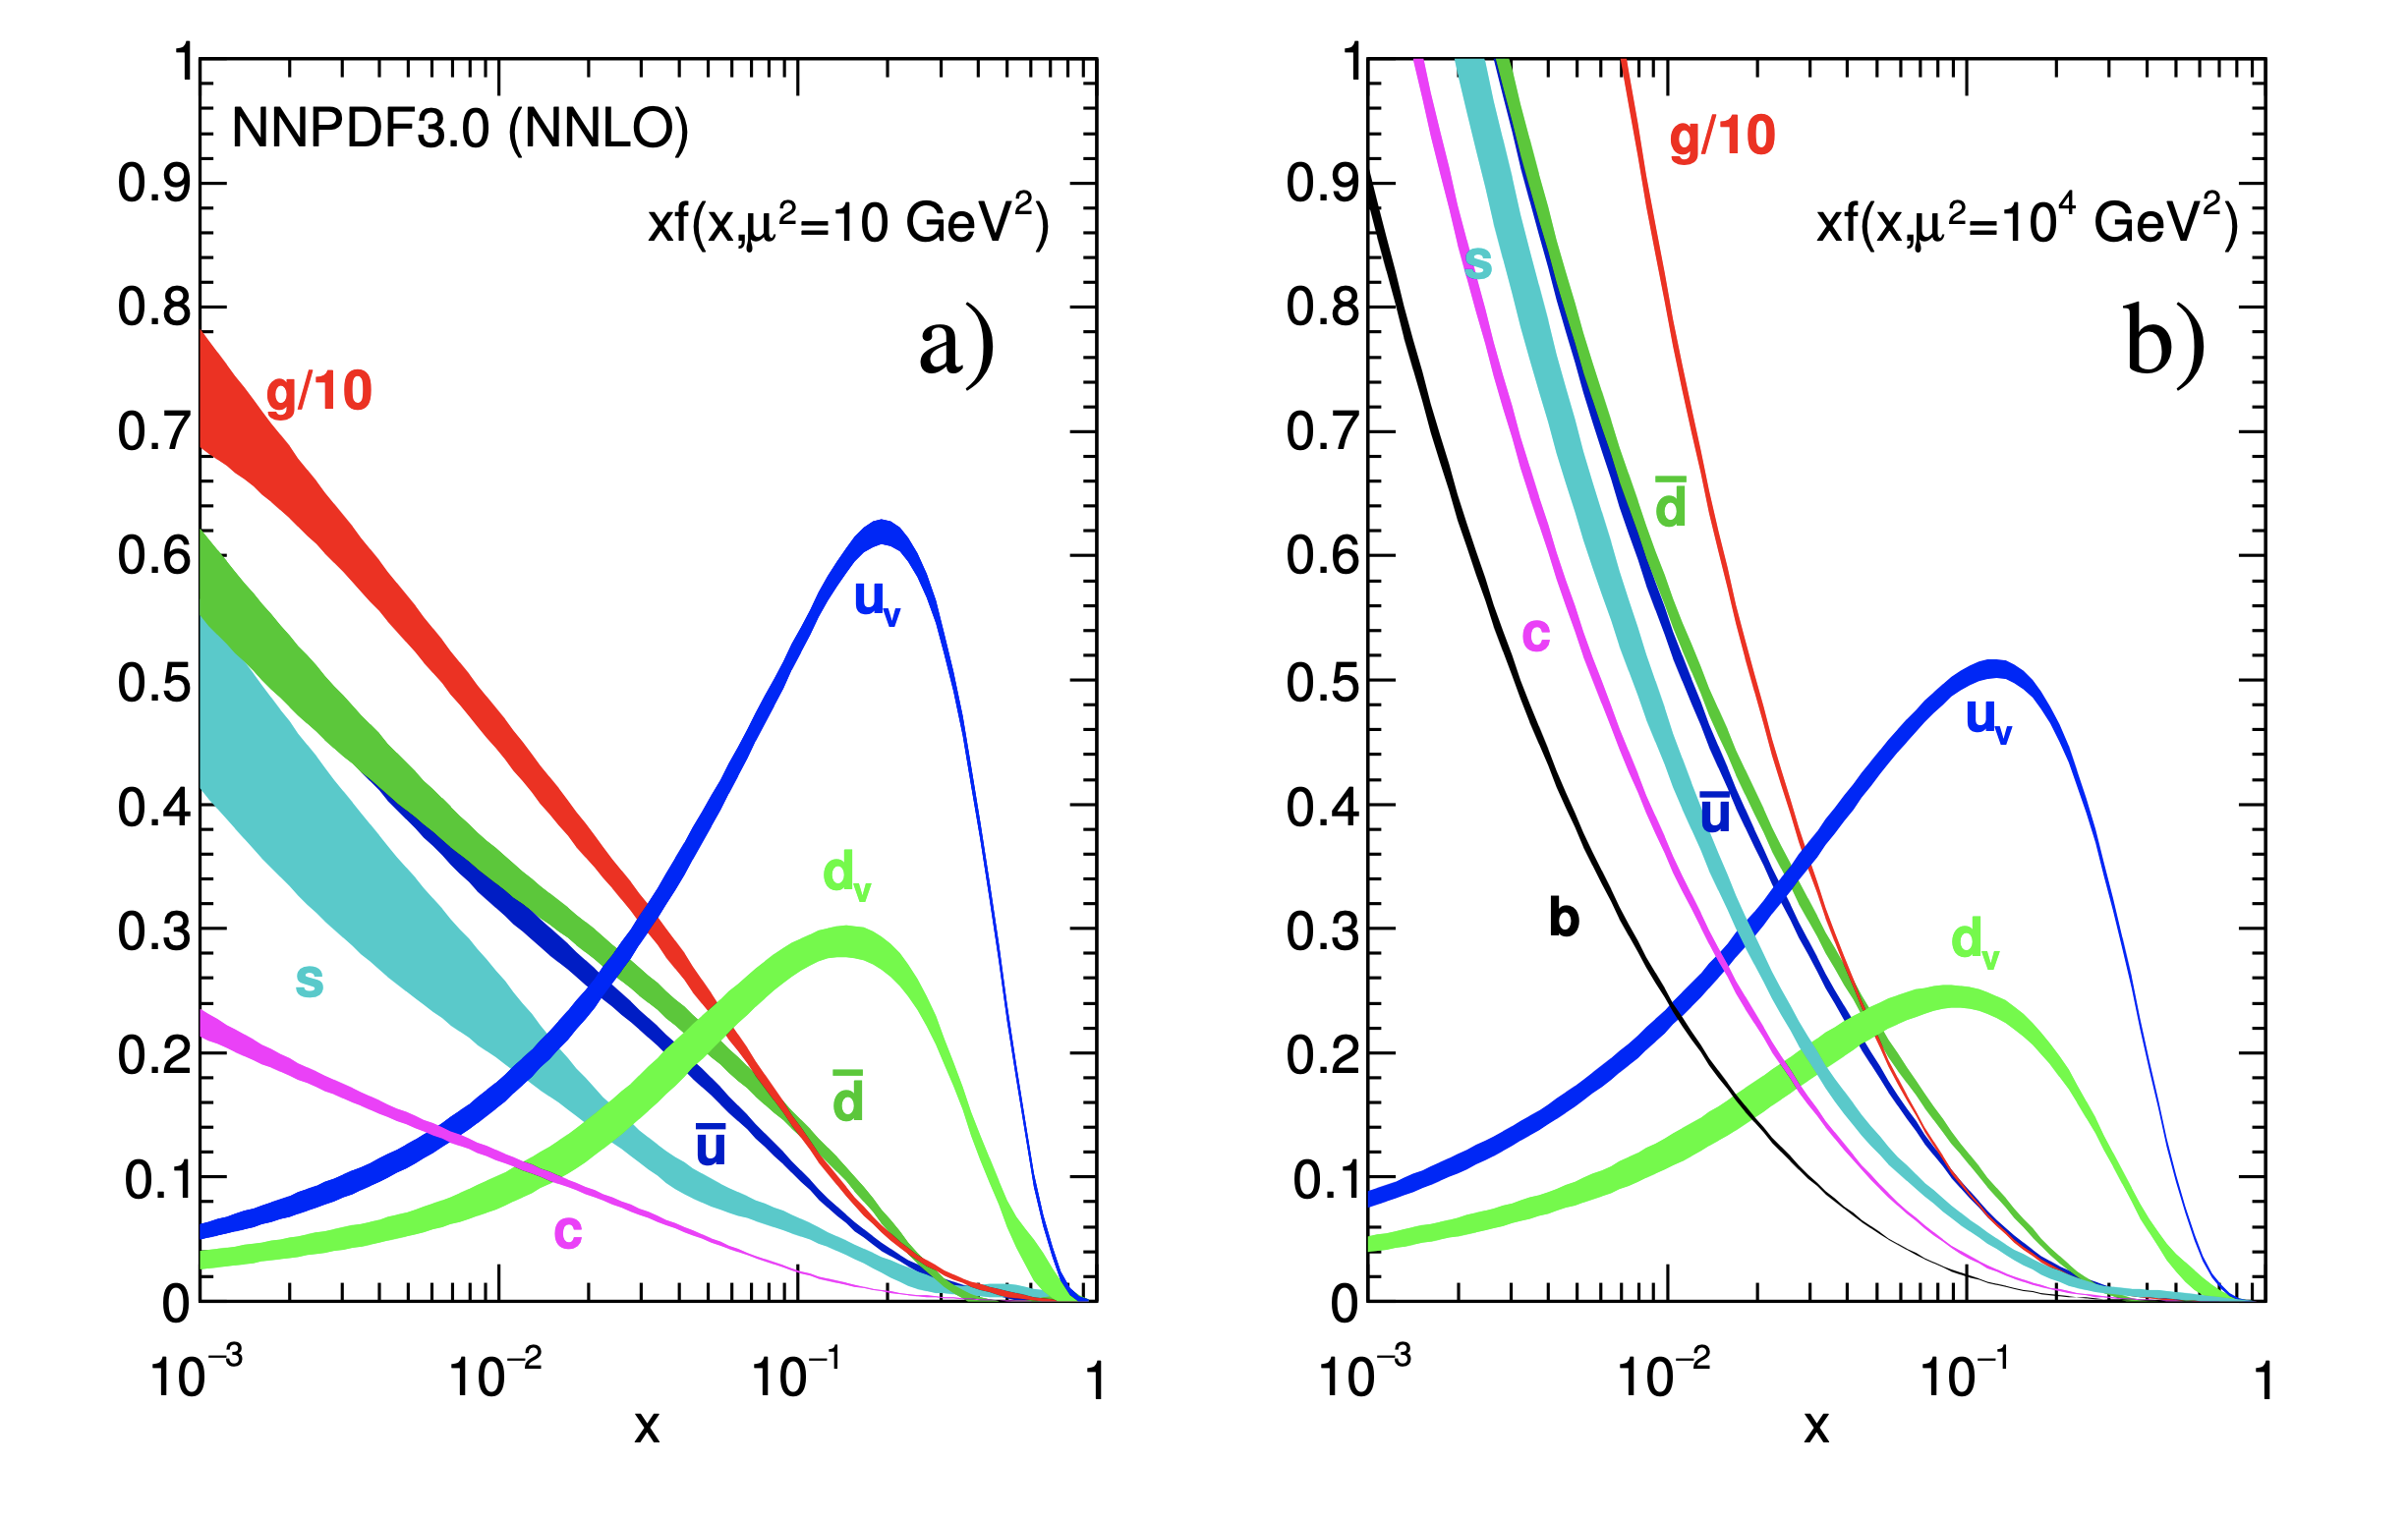
\includegraphics[width = 0.7 \textwidth]{chapters/RelatedWorks/sectionPPCollision/figures/pdf.png}
    \caption{PDF of valence quark, sea quark and gluon at $\mu^2=10 \text{ GeV}^2$ and $\mu^2=10^4 \text{ GeV}^2$. The valence quarks dominate the high-x region and in total only account for about 38\% of the proton momentum. The low-x region is dominated by the sea quarks and gluons, forming a ``soft cloud'' around the valence quarks inside the proton. Gluons are the major components of the ``soft cloud'', and in total carry over 40\% of the proton momentum. Comparing PDF in a) and b), the increasing of the energy scale dramatically populates the soft gluons and soft sea quarks.  Intuitively speaking, more and more ``soft cloud" of sea quarks and gluons are revealed as the probing energy increases.}
    \label{fig:relatedWorks:ppCollision:pdf}
\end{figure}



\subsection{Hard Process}
\label{sec:relatedWorks:ppCollision:hardProcess} 


The hard process of partons happens in a short-distance range and can be calculated with perturbative quantum field theories. In the LHC, the hard processes allowed by the SM include the EW, QCD, and Higgs interactions. Figure~\ref{fig:relatedWorks:ppCollision:hardxs} shows a summary of the total cross-section of the SM processes in the LHC measured by the experiments and predicted by the SM. For this thesis, the signal processes include a pair of W bosons, namely $t\bar{t}$, $tW$, and $WW$ productions.




\begin{figure}[ht]
    \centering
    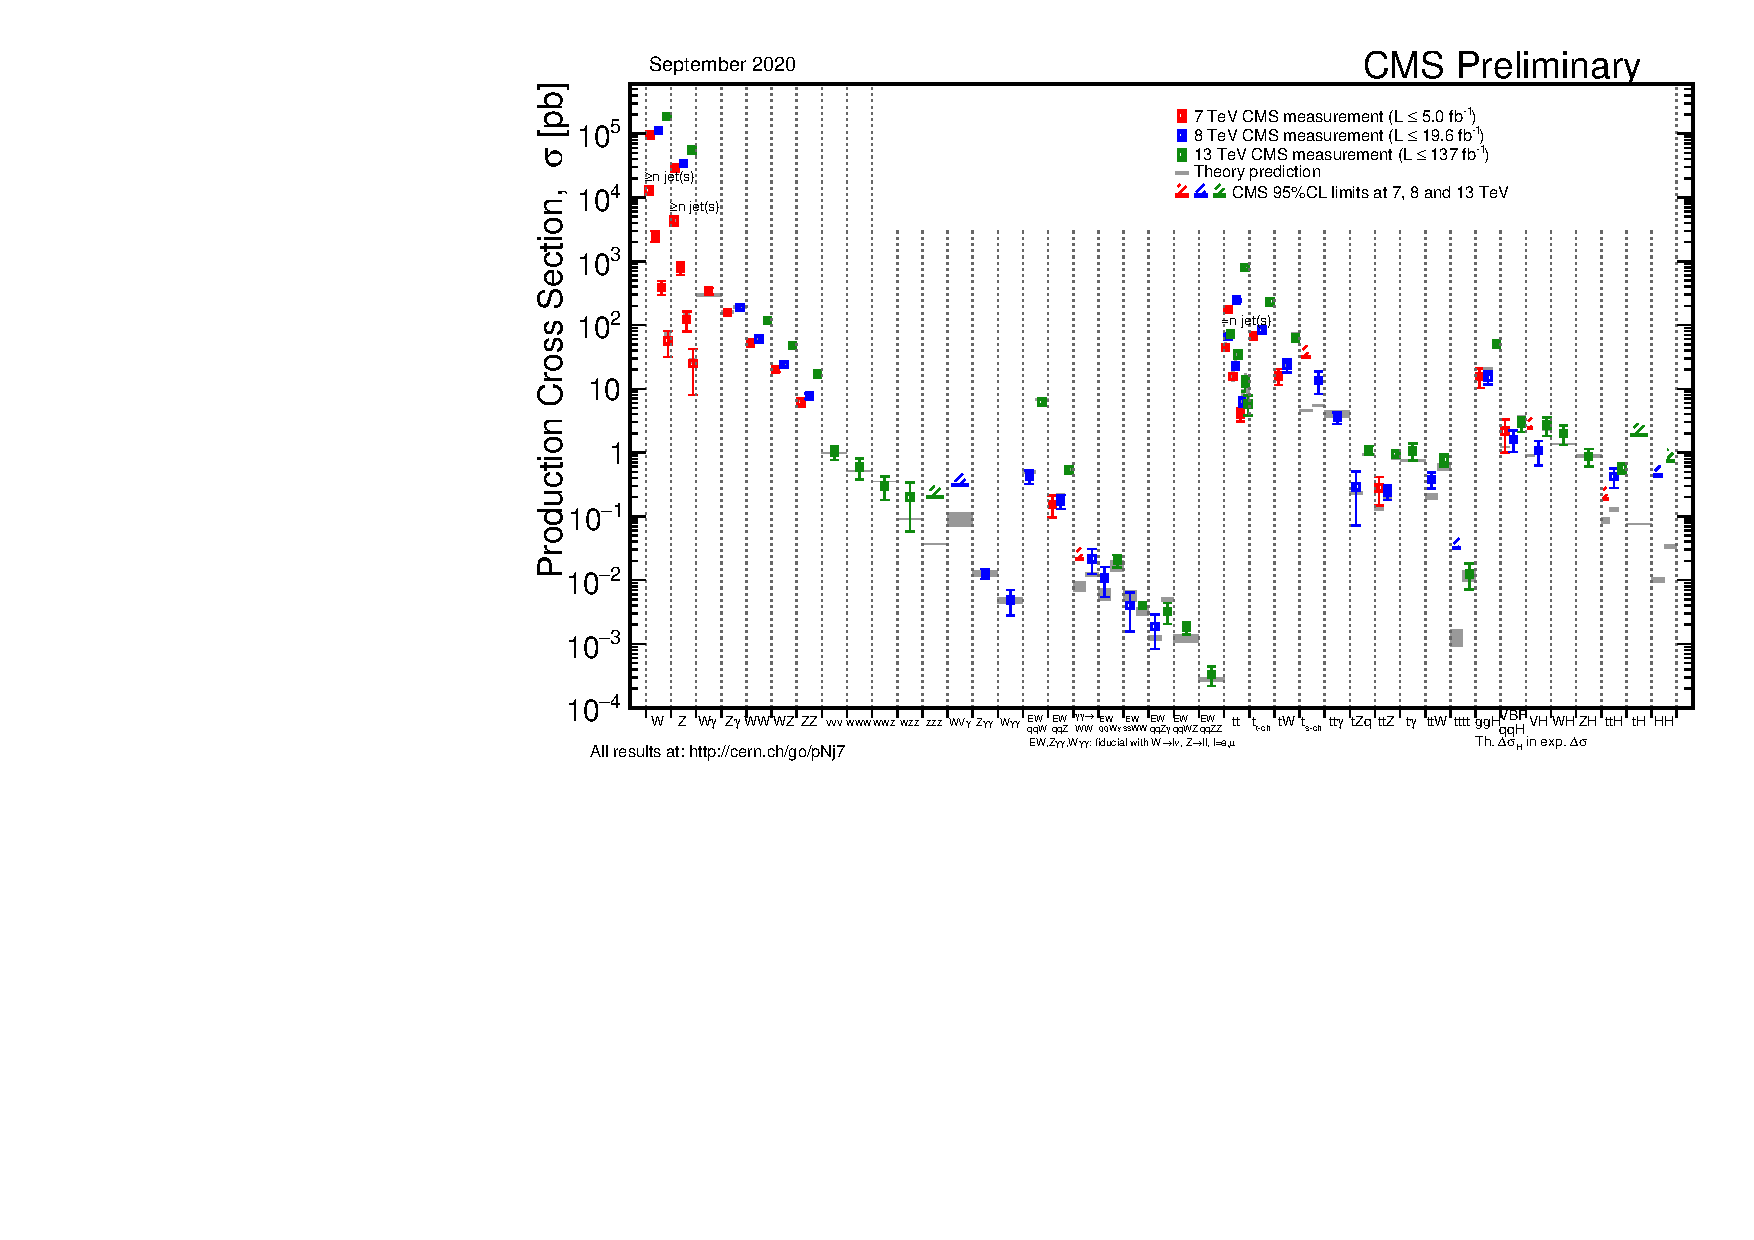
\includegraphics[width=0.99\textwidth]{chapters/RelatedWorks/sectionPPCollision/figures/SigmaNew_v0.pdf}
    \caption{Summary of the cross-sections of the SM process in the LHC. The grey bar shows the theoretical prediction. The red, blue and green shows the CMS measurement or the excluded limit at 7, 8, 13 TeV.}
    \label{fig:relatedWorks:ppCollision:hardxs}
\end{figure}

% \begin{figure}
%     \centering
%     \includegraphics[width=0.6\textwidth]{smXs.pdf}
%     \caption{Caption}
%     \label{fig:my_label}
% \end{figure}

\begin{figure}[ht]
    \centering
    \feynmandiagram[small,horizontal=a to b]{
        i1 [particle=\(q\)] -- [fermion] a -- [fermion] i2 [particle=\(q\)],
        a -- [gluon, edge label=\(g\)] b,
        f1 [particle=\(t\)] -- [fermion] b -- [fermion] f2 [particle=\(t\)],
        % top decay
        f1b[particle=\(b\)] -- [fermion] f1 -- [photon] f1W [particle=\(W\), red],
        f2b[particle=\(b\)] -- [anti fermion] f2 -- [photon] f2W [particle=\(W\), red],
        f1 -- [opacity=0.0] f2,
        f1W -- [opacity=0.0] f2W,
        f1b -- [opacity=0.0] f1W,
        f2b -- [opacity=0.0] f2W,
    }; \qquad
    \feynmandiagram[small,horizontal=a to b]{
        i1 [particle=\(g\)] -- [gluon] a -- [gluon] i2 [particle=\(g\)],
        a -- [gluon, edge label=\(g\)] b,
        f1 [particle=\(t\)] -- [fermion] b -- [fermion] f2 [particle=\(t\)],
        % top decay
        f1b[particle=\(b\)] -- [fermion] f1 -- [photon] f1W [particle=\(W\), red],
        f2b[particle=\(b\)] -- [anti fermion] f2 -- [photon] f2W [particle=\(W\), red],
        f1 -- [opacity=0.0] f2,
        f1W -- [opacity=0.0] f2W,
        f1b -- [opacity=0.0] f1W,
        f2b -- [opacity=0.0] f2W,
    }; \qquad
    \feynmandiagram[small, vertical=a to b, horizontal=a to f1]{
        i1 [particle=\(g\)] -- [gluon] a -- [anti fermion] f1 [particle=\(t\)],
        a -- [fermion, edge label=\(t\)] b,
        i2 [particle=\(g\)] -- [gluon] b -- [fermion] f2 [particle=\(t\)],
        % top decay
        f1b[particle=\(b\)] -- [fermion] f1 -- [photon] f1W [particle=\(W\), red],
        f2b[particle=\(b\)] -- [anti fermion] f2 -- [photon] f2W [particle=\(W\), red],
        f1 -- [opacity=0.0] f2,
        f1W -- [opacity=0.0] f2W,
        f1b -- [opacity=0.0] f1W,
        f2b -- [opacity=0.0] f2W,
        % i1 -- [opacity=0.0] i2,
        % f1 -- [opacity=0.0] f2,
    };
    \caption{The tree-level process of $t\bar{t}$ production in the LHC. In all three diagrams, $t\bar{t}$ is produced with the QCD interaction. In the LHC, the dominant production processes are the two diagrams on the right, with two incoming gluons colliding in the s-channel and t-channel, respectively. The top quark decays into W boson and b quark immediately after production.}
    \label{fig:relatedWorks:ppCollision:tt}
\end{figure}

\noindent In the hadron collider, top quark pairs are produced with the QCD interaction. The tree-level diagrams for the $t\bar{t}$ production is shown in Figure~\ref{fig:relatedWorks:collider:tt}. The quark-antiquark annihilation, shown as Figure~\ref{fig:relatedWorks:ppCollision:tt} left, was the dominant process in the Tevatron, where the quark and antiquark are the valence quark in the proton and anti-proton, respectively. But in the LHC, which collides proton-proton at higher center-of-mass energy, gluon-gluon fusion in the s channel and t channel, shown as  Figure~\ref{fig:relatedWorks:ppCollision:tt} middle and right, are the dominant diagrams. The top quark decays into a b quark and a W boson instantly after produced. The resulting pair of W bosons are used to measure $Br(W)$ in this thesis. Meanwhile, the outcoming b quarks are used to tag these signal events. The theoretical prediction of tt cross-section at 13 TeV LHC is
\begin{equation}
    \sigma_{tt} = 831.76 ^{+19.77}_{-29.20} \text{ (scale) } \pm 35.06 \text{ (PDF, $\alpha_s$) pb } .
\end{equation}



\begin{figure}[ht]
    \centering
    \feynmandiagram[small,horizontal=a to b]{
        i1 [particle=\(b\)] -- [fermion] a -- [gluon] i2 [particle=\(g\)],
        a -- [fermion, edge label=\(b\)] b,
        f1 [particle=\(W\) , red] -- [photon] b -- [fermion] f2 [particle=\(t\)],
        f2b[particle=\(b\)] -- [anti fermion] f2 -- [photon] f2W [particle=\(W\), red],
        f1 -- [opacity=0.0] f2W,
    }; \qquad
    \caption{The tree-level process of tW production. The incoming b quark scatters off a gluon with QCD interaction and gets excited into top quark and W boson via EW interaction.}
    \label{fig:relatedWorks:ppCollision:tw}
\end{figure}

\noindent The tW production is induced via the weak interaction and thus has smaller cross-section comparing the top pair production. The tree-level tW production process is shown in Figure~\ref{fig:relatedWorks:ppCollision:tw}. One of the W boson is produced associated with top quark. The outcoming top quark decays into a b quark and another W boson. The two W bosons are used for  $Br(W)$ measurement, while the b quark is used to tag $tW$ events. The SM theoretical cross section for tW is 
\begin{equation}
    \sigma_{tW} = 71.7 \pm 1.80 \text{ (scale) } \pm 3.40  \text{ (PDF, $\alpha_s$) pb }
\end{equation}


\begin{figure}[ht]
    \centering
    \feynmandiagram[small,horizontal=a to b]{
        i1 [particle=\(q\)] -- [fermion] a -- [fermion] i2 [particle=\(q\)],
        a -- [photon, edge label=\(Z\)] b,
        f1 [particle=\(W\), red] -- [photon] b -- [photon] f2 [particle=\(W\), red],
    }; \qquad
    \feynmandiagram[small, vertical=a to b, horizontal=a to f1]{
        i1 [particle=\(q\)] -- [fermion] a -- [photon] f1 [particle=\(W\), red],
        a -- [fermion, edge label=\(q''\)] b,
        i2 [particle=\(q'\)] -- [anti fermion] b -- [photon] f2 [particle=\(W\), red],
        i1 -- [opacity=0.0] i2,
        f1 -- [opacity=0.0] f2,
    };
    \caption{The Tree-level process of WW production. These two diagrams are both induced by the electroweak interaction. }
    \label{fig:relatedWorks:ppCollision:ww}
\end{figure}

\noindent The WW production by EW interactions. Figure~\ref{fig:relatedWorks:ppCollision:ww} shows two major tree-level processes for the WW production. In the first diagram, quark-antiquark annihilates into a virtual $Z/\gamma$, which then decays into WW pair via EW triple-gauge-coupling. In the second diagram, WW is produced in the t-channel of quark-quark scattering. The WW process contributes to the event selection without b-tags. But the contribution is small due to its small cross-section. The treatment of the WW process is different between the shape analysis and the counting analysis: the shape analysis utilizes W bosons in the WW process as a signal, while the counting analysis treats it as a background. The SM theoretical cross-section for WW is 
\begin{equation}
    \sigma_{WW} = ?? \pm ??  \text{ (scale) }  \pm ??  \text{ (PDF, $\alpha_s$) pb }
\end{equation}


\subsection{Fragmentation}
\label{sec:relatedWorks:ppCollision:psJet} 

Quarks and gluons from the hard process are colored, but only the colorless particles can finally reach the detector. A few processes of the outcoming partons take place between the hard process and the particle reaching the detectors. These processes mainly include the parton shower, hadronization, and decay. In an energy scale $Q>\Lambda_{QCD}$, the quarks emit gluons, and subsequently, gluons convert into quark-antiquark pairs. An initial parton ends up with a bunch of secondary partons. And the initial momentum is split among all the secondary partons. This process is called the parton shower. The differential phase space of the gluon emission is
\begin{equation}
    dS = \frac{2\alpha_s C_F}{\pi} \frac{dE}{E}\frac{d\theta}{\sin \theta} \frac{d\phi}{2\pi}.
\end{equation}

\noindent The gluon emission diverges at a small $\theta$ or a small energy $E$, often referred to as ``inferred colinear" divergence. Therefore the parton shower tends to soft and colinear within a narrow cone of the initial parton. But these divergences are canceled by the contributions from virtual diagrams, discussed in Section~\ref{sec:relatedWorks:vcs}, resulting in a finite total cross-section of the gluon emission. When the energy scale of the parton shower drops below $\Lambda_{QCD}$, the partons start to group together and forms into mesons and baryons, which is called hadronization. There are two popular models for the hadronization process, the cluster approach and the string approach, both of which contain a few algorithm parameters usually tuned with the experimental data. For example, Pythia8 uses the string model for hadronization tuned with LEP and LHC Run1 data. Parton shower plus hadronization is often referred to as the ``fragmentation''. After the fragmentation, unstable mesons and baryons decay into stable particles like $\pi, K, \gamma, e, \mu, $, following the corresponding life-times and certain decaying matrix elements, such as EW decaying matrix element. The decay process can be also handle by Pythia8.

The parton from the hard process, after parton shower, hadronization, and decay, finally ends up to be a narrow cone of stable particles, including charge hadrons, neutral hadrons, photons, and leptons. This cone of particles can be clustered together to represent the initial seeding partons. This cluster of colinear particles is called a jet. A jet is defined by a clustering algorithm (e.g. anti-kt) and scale parameter (e.g. $\delta R=0.4$). To reliably represent the seeding parton, a jet algorithm has to be  insensitive to the soft-colinear parton showering, so-called ``inferred colinear safe''. The jet reconstruction in the CMS is discussed in Section XXX (CMS detector).

